\documentclass{jarticle}
\usepackage{lmodern}%(Latin Modern font)
\usepackage[T1]{fontenc}
\usepackage{amsmath}
\usepackage{amssymb}
\usepackage{bm}
\usepackage[dvipdfmx]{xcolor}
\usepackage[dvipdfmx]{graphicx}
\usepackage{apmayfes2015}
\usepackage[top=30truemm,bottom=30truemm,right=25truemm]{geometry}
\title{ICAを用いたカクテルパーティー効果}
\author{計数工学科数理情報コース B4 八嶋晋吾}
\date{}

\begin{document}
\maketitle
\section{キーワード}
\begin{itemize}
  \setlength{\parskip}{0cm}
  \setlength{\itemsep}{0cm}
  \item 信号処理
  \item 独立成分分析・ICA
  \item カクテルパーティー効果
\end{itemize}

\section{理論解説}
\subsection{独立成分分析(ICA)とは}
独立成分分析(ICA: Independent Component Analysis)とは,多変量のデータから隠された因子や成分を見つけ出すための
一手法である.より具体的には,複数の信号が混合して観測されたものから「元の信号が統計的に独立である」
という仮定のみを用いてそれぞれの信号を推定する.\par
他の一般的な分析手法である因子分析や主成分分析(PCA)は,各成分が無相関になるように信号を分離する.原信号がガウス信号であれば「無相関$\Leftrightarrow$独立」
が成り立つため,それらの手法を用いて信号を独立な成分に分離することができるが,一般に現実の音声は非ガウス的な信号であることが多く,それでは不十分である.
そこでICAは,原信号が非ガウス的な場合において各成分が独立になるように分離することを可能にしている.\par
図1に3種類の信号から生成した混合信号からICAとPCAを用いて原信号を推定したものを示す.ICAではほぼ完全に原信号を復元できているが,PCAはできていないことがわかる.
\begin{figure}[htbp]
\begin{center}
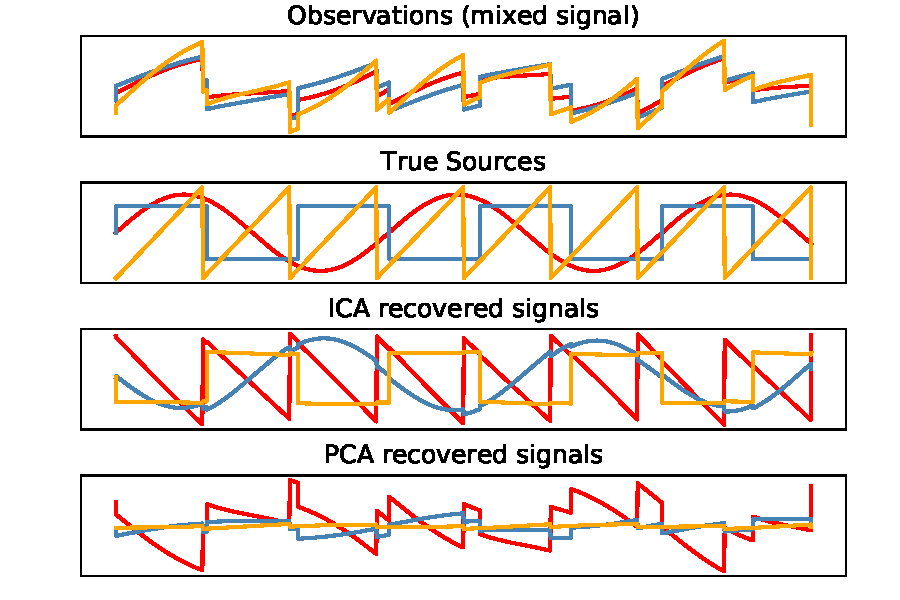
\includegraphics[clip,width=10.5cm]{./ica.pdf}
\caption{ICAとPCAを用いた信号推定}
\end{center}
\end{figure}
%ICAで推定する際の制約としては「原信号が非ガウス的であること」「混合信号の数と原信号の数が等しいこと」がある.

\subsection{ICAの制約条件}
ICAによる信号推定が可能になるためには,以下の条件を満たす必要となる.
\begin{itemize}
  \setlength{\parskip}{0cm}
  \setlength{\itemsep}{0cm}
  \item 信号源のうち,高々ひとつだけがガウス雑音であること.
  \item 観測された混合信号の数が,原信号の数と等しいか,それより多いこと.
  \item 各混合信号について,原信号の重みベクトルが一次独立であること.
\end{itemize}\par
よってICAをカクテルパーティー効果に用いる場合,話者の人数分の混合音源が必要になる.

\subsection{アルゴリズム}
観測信号は原信号の線型結合と考えられるから,同様に原信号$y$は観測信号$\bm{x}$の線型結合として$y = \trsps{\bm{b}}\bm{x}$と表すことができる.
独立成分を求める問題は,最適な重み$\bm{b}$を求める問題と等価である.\par
中心極限定理より,独立な信号を混合したものは元の信号よりもガウス分布に近くなる.つまり,観測信号$\bm{x}$の線型結合$y$
で,非ガウス性が高くなるものが独立成分の一つであると考えることができる.\par
非ガウス性を測るパラメーターとしては,信号の尖度が用いられる.確率変数$y$の尖度とは,4次のキュムラントのことであり
\begin{equation}
\mathrm{kurt}(y) = \mathrm{E}\{y^4\}-3(\mathrm{E}\{y^2\})^2\nonumber
\end{equation}
と定義される.$y$がガウス分布に従うとき,$\mathrm{kurt}(y)=0$となるため,$|\mathrm{kurt}(y)|$を最大化することで$y$の非ガウス性を最大化することができる.\par
以上をまとめると,信号の独立成分を求める問題は,重み$\bm{b}$を変数として$|\mathrm{kurt}(\trsps{\bm{b}}\bm{x})|$の極値を求める問題に帰着させることができる.実際に勾配降下法や
高速不動点アルゴリズムを用いることで,その極値を求めることが可能である.\par
ここでは独立性を最大化する規範として,非ガウス性の最大化を用いた方法を解説した.他にも最尤推定を用いた方法や,相互情報量を最小化する方法があるが,ここでは割愛する.





\subsection{周波数領域でのICA}
実際に信号を観測する際には,ノイズや残響も入力される.特に今回の展示のように部屋の中で音声を観測する場合,残響の影響はかなり大きくなる.
さらに,音源からの信号はマイクの位置により異なる時間差で到達するため,時間領域でのICAでは上手く原信号を推定することができない.\par
このような場合の混合信号は時間領域での畳込みでモデル化されるため,フーリエ変換することにより混合信号を原信号の線型結合として表すことができる.そこで
観測信号をフーリエ変換したのち,周波数領域でICAを行うことで原信号を推定することができる.

\section{実装}


\section{応用例}
\begin{itemize}
  \setlength{\parskip}{0cm}
  \setlength{\itemsep}{0cm}
  \item カクテルパーティー効果\\
  複数人が同時に話した音声をICAにかけることで,それぞれの人の音声を分離することができる.
  \item 脳機能の可視化\\
  脳の外部から観測される脳波や脳磁図は,脳の内部の複数の信号源からの混合信号だと考えることができるため,
  観測信号から脳の活動部位を可視化することができる.
  \item 画像の特徴抽出\\
  画像データをICAにかけ,基底ベクトルを推定することにより,画像のスパースな表現を得ることができる.これは
  データ圧縮や雑音除去に応用可能である.

\end{itemize}

\begin{thebibliography}{9}
  \bibitem{a} A.Hyvarinen, J.Karhunen, E.Oja, 『詳解 独立成分分析』, 東京電機大学出版局, 2005
  \bibitem{b} 浅野 太, 電子情報通信学会『知識の森』2群6編2章『音源分離』, 2011
  \bibitem{c} 五反田 博, 石橋 孝昭, 岩崎 宣生, 井上 勝裕, "独立成分分析の基礎と応用", 2011
\end{thebibliography}

\end{document}
